\begin{savequote}[75mm]
Talk is cheap. Show me the code.
\qauthor{Linus Torvalds}
\end{savequote}

\chapter{Software for Velo daily operation}
\label{chap:software}

The development of the Large Hadron Collider was foreseen in steps, consisting of data-taking runs and technical stops.
Since the radiation may cause damage to the parts of the accelerator as well as to the parts of the detectors, these interruptions are necessary not only to mitigate the radiation damage but to provide a window of opportunity for the upgrade of the composition of the detectors.
Since many of the procedures that rely on the detectors are tailor-fitted to the devices, parts of the software created for previous versions of the hardware cannot be possibly used for the upgraded setup.
The Storck project was created because of the lack of a system for handling and tracking of the calibration data. The Titania project was designed and implemented in place of the old monitoring system called Lovell.

\section{Storck}

Storck stands for ``Data \textbf{Stor}age and Tra\textbf{ck}ing''. It is a database system created to store Velo calibration data.
It was developed using python \cite{10.5555/1593511} and Django framework \cite{django}.
At the time of writing, it is being adapted at CERN for use in the commissioning of upgraded Velo pixel detector and subsequently in its daily operation.
This section will present its design.
The implementation details can be referred to in the CERN's GitLab repository \cite{bworld} and online documentation page\cite{storckdock}.

\subsection{Motivation}

The scientific workflow when preparing or managing a high energy particle detector requires taking vast amounts of different types of data.
Apart from the immediate data coming from the device, other data types, such as detector's condition (sensors' temperature, date, and duration of the run), are also needed.
The development of the monitoring process might be messy and evolve in time.
This is also true for the monitoring tasks when using the detector for taking physical data.
Usually, data storage problems are solved with relational databases.
But, the relational databases require a predefined structure that is not easy to be modified when the data have been uploaded.
Relational and non-relational databases are both inefficient for storing large binary files.
For those reasons, the Storck project was created.
It utilises a relational database with non-relational elements using the filesystem storage.
It is not oriented towards one type of file, nor does it expect any kind of predefined structure.
Storck allows to share data between its users and track the changes in the data.


\subsection{Software stack}

The software stack of the Storck project reflects the newest trends in the enterprise software development, as well as best practices in the industry.

\subsubsection{Django and Django rest API}
Python language provides many web frameworks.
One of the most popular of them is Django \cite{django}. 
Django is a mature web design framework based on the Model-View-Controller (MVC) design pattern.
Django is split between Model, View and Template.
It is important to note that functionally Django View corresponds to Controller and Template to View parts of MVC.
This design pattern allows for logical separation of the functional responsibility of the code.
Functionality of a Django project are encapsulated in, so called, applications.
Each of the application implements its own version of MVC, though it is possible to use any of the components of the MVC design from any other application.
This framework also utilises object-relational mapping, which frees the framework user from writing queries using SQL language, and allows for high-level object-oriented usage of the model.

\subsubsection{PostgresSQL}
PostgresSQL \cite{postgres} is a widespread implementation of a relational database. It is SQL compliant. Importantly, it is free and open source. A recent version introduced a non-relational capability, which is storing the JSON data format along with the ability to make queries using JSON data format.

\subsubsection{Docker}

Docker \cite{merkel2014docker} provides OS-level virtualisation. It uses images and containers. Docker image is a software package that contains everything necessary to run an application.
Images are defined in special files called Dockerfiles. Image definition is done by using Dockerfile commands.
Images are usually based on operating systems, like Ubuntu Linux or Alpine Linux.
The former is the most popular choice, as the base image from alpine Linux needs only 8 MB of disk space.
When Images are being mounted to the docker daemon, they are referred to as containers.

\subsection{Service Design Overview}

The system's design at heart uses REST API communication for managing the access to the database.
Users have multiple ways of interacting with Storck, but all of them internally use REST API.
Users can use the web interface and manually input or download the data.
For convenience, a python wrapper to the REST API also exists, so users can easily create scripts that will interact with Storck.
When the webserver receives commands via REST API, it interacts with PostgresSQL to validate the request and responds using an HTTP request, either by providing the requested information (like a list of files, file details) or by sending the file.
Because HTTP servers may be a bottleneck when serving large amounts of data, we implemented the possibility of downloading the data using direct files access.
When storing files, Storck doesn't write them directly to the database, but it saves them to the disk.
By the design of the CERN's computing ecosystem, this disk space is accessible by ssh connection with the CERN's lxplus servers.
The Fig. \ref{fig:storck_diagram} contains a schematic diagram for the data flow in the Storck.


\begin{figure}[H]
\centering
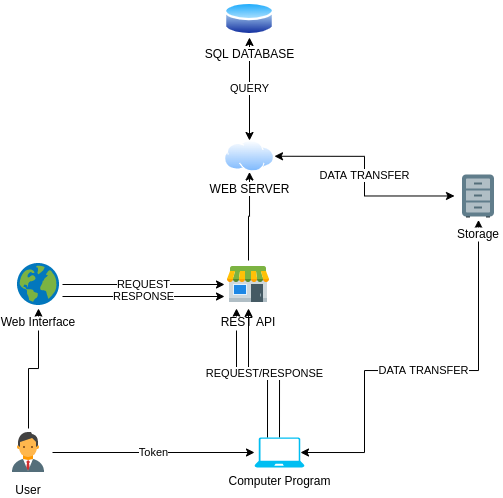
\includegraphics[width=0.95\textwidth]{figures/chapter5/storck/storck diagram.drawio.png}
\caption{The conceptual chart of the data flow in the Storck service.}
\label{fig:storck_diagram}
\end{figure}

\subsection{Implementation}

The overall implementation spans over a few Django applications. I will not present parts of the code here, as I feel this would be excessive.
Yet we provide an overview of the essential parts of the implementation of the service.

\subsubsection{Files}

\begin{table}[h]
\begin{center}
\begin{tabular}{ |c|c| }
\hline
Property & Django model type \\
\hline
id & AutoField \\
file & FileField \\
hash & TextField \\
workspace & ForeignKey \\
user & ForeignKey \\
previous\_version & ForeignKey \\
duplicate\_of & ForeignKey \\
date & DateTimeField \\
fake\_path & TextField \\
meta\_open & JsonField \\
meta\_closed & TextField \\
hide & BooleanField \\
\hline
\end{tabular}
\caption{\label{tab:storck_filesfield}Table of contents of the StorckFile model.}
\end{center}
\end{table}

The most crucial element of the Storck is the StorckFile model/database. It keeps track of the uploaded files and stores additional information and metadata.
The \textit{id} field contains a unique identifier that identifies each of the files in the database.
Next, the \textit{file}, which is of Django's File field type, contains a path to a locally saved file.
This property is not implicitly created as the request to file with its contents comes in, but instead, it is designed with the deduplication procedure described in Sec \ref{sec:deduplication}.
\textit{Hash} is the md5sum of the file's contents, calculated upon receiving.
\textit{Workspace} and \textit{user} contain a foreign key connection to the list of all workspaces and users.
The \textit{User} field contains the user id of the user who uploaded this file (or its duplicate).
\textit{Previous\_version} points to the record containing the previous version of the given file.
Here ``new version'' means a new file in a given workspace with the same \textit{fake\_path} attribute.
\textit{duplicate\_of} contains a reference to the file's duplicate record.
\textit{fake\_path} is the logical path of the file.
This property has no physical sense for the Storck database, as the files are not stored using this path.
\textit{meta\_open} is the metadata property.
It is JsonField, which makes it flexible, and allows to create an arbitrary structure of the data inside the field.
Because we don't want to show older versions of files in the web view, we use flag \textit{hide} to decide whether the file is shown or not.


\subsubsection{Authentication}
The CERN account system allows for OAuth 2.0 \cite{rfc6819} authorisation for third party services.
Each person in CERN has a personal CERN account that identifies the user.
It uses an (OIDC) OpenID Connect system built on top of the OAuth 2.0 framework.
That means that instead of requiring a proprietary login password in Storck, we can redirect the login to CERN SSO (CERN single sign-on) service.
There, user can use their CERN Account password and log in, the same that is being used for other services at CERN to log in.
Automatically, in the background, CERN SSO communicates to the web server and confirms the user's identity.
Setting up the authentication with OIDC requires setting proper tokens on the administrator side. Those can be generated using the CERN application portal.
Although we refer to CERN's authentication procedures in this section, for anyone willing to reuse Storck for other purposes, it is possible to do that with any authentication system that implements the OIDC.
None of the parts of this process is specifically dedicated only to the CERN ecosystem, as OIDC can be interfaced with other services that provide authorisation.


\subsubsection{Deduplication}
\label{sec:deduplication}

The deduplication process is used when the file is about to be saved in the Storck.
The server must receive the file's content, and when the process is finished, the server calculates the md5sum hash value.
The database is then checked for the hash matching the file.
If the same hash exists in the database, then the record containing this hash is the duplicate of the incoming file.
If the file has no duplicate, it is processed and saved normally.
But if the duplicate exists, the received file content is discarded.
The entry to the file database progresses normally, and the file path to the incoming file is set to be the same as the already existing file.
Additionally, the attribute \textit{duplicate\_of} is also set to point to the \textit{id} of the entry of the existing file record.

\subsection{REST API}

The REST API makes for a perfect interface for projects like this.
Most modern programming languages are capable of making HTTP requests by themselves, and there CERN already utilises an extensive internal network.
REST API is agnostic of an operating system and programing language.
In my previous experience with LHCb monitoring, one of the biggest challenges was the compatibility of the database tools, which only interfaced with the C++ library.
The design of STORCK is free of this problem, as the client of the system doesn't need to update every time there is a change in the Storck service.


\begin{figure}
\resizebox{0.5\columnwidth}{!}{%
\begin{tabular}{ c c c }
\hline
method & path & params \\
\hline
GET & /api/workspaces &  \\
\hline
POST & /api/workspace & name (body) \\
\hline
POST & /api/workspace/user & workspacetoken (body) \\
 & & userid (body)
 \label{tab:workspace-api}
\end{tabular}
}
\quad
\resizebox{0.4\columnwidth}{!}{%
\begin{tabular}{ c c c }
\hline
method & path & params \\
\hline
GET & /api/files & hidden (query) \\
 & & token (query) \\
\hline
 GET & /api/file & info (query) \\
 & & id (query) \\
 & & token (query) \\
\hline
 POST & /api/file & token (query) \\
 & & file (body) \\
 & & path (body) \\
 & & meta (body)
  \label{tab:file-api}
\end{tabular}
}

\label{tab:storck_rest_api}
    \caption{ Workspace endpoints of the REST API and their parameters (left) and the endpoints for interaction with Storck files (right). }
\end{figure}

Tab. {tab:workspace-api}, {tab:file-api}, present the listing of the REST API methods.
The first endpoint provides a way of creating and managing the workspaces. That includes the creation of the workspace, getting workspaces information, and its associated user list.
The second endpoint is responsible for searching for the file, downloading and uploading, and getting detailed information about the files.

\subsection{Deployment}

The novel deployment process standard in the IT industry is using Dockerisation.
And so, Storck, in its deployment, depends on it.

\begin{figure}[H]
\centering
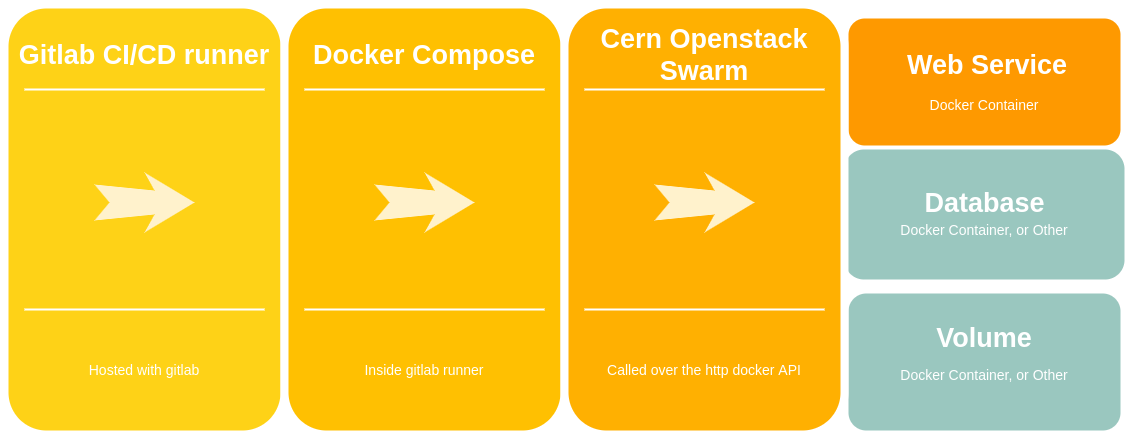
\includegraphics[width=0.95\textwidth]{figures/chapter5/storck/storck_dockers.drawio.png}
\caption{The schematic of the Storck deployment process. The light green colour means optional components.}
\label{fig:storck-dockers}
\end{figure}

The Fig. \ref{fig:storck-dockers} depicts the flowchart of the deployment for storck.
The lowest level of the deployment consists of 3 docker images, Web App, Database and Volume.
The last two are optional as, in fact, it is possible to use external (not dockerised) Volume and external Database service.
A database can be run simply by using a predefined docker image.
Web App is created using a custom Dockerfile.
The base image is the Alpine Linux image with python 3.8.
During the building of the image, it set's up necessary environment variables, dependencies, and migrations, and in the end, runs the uwsgi server.

\subsection{Gitlab CI}

As visible in the Fig. \ref{fig:storck-dockers}, the Gitlab CI run environment is the first part of the deployment process.
Although GitLab started purely as a service that allows for hosting and browsing the git repositories, like many other git services, it provides a mechanism for Continous Integration / Continuous Deployment.
It means that there is no longer a need for a dedicated server that will be running a test environment and enables manual triggering of some deployment or testing jobs just after committing to the repository.
It is now perfectly possible to do those things from the GitLab web interface.

\begin{figure}[H]
\centering
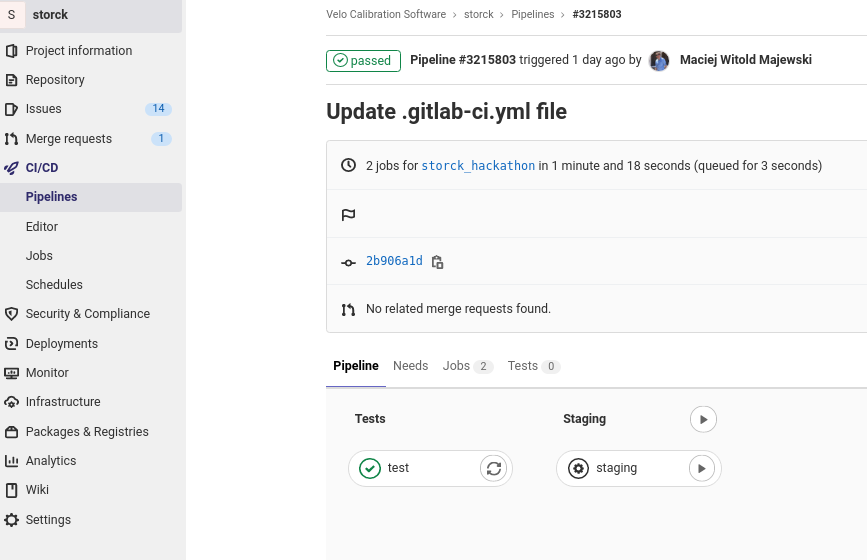
\includegraphics[width=0.95\textwidth]{figures/chapter5/storck/storck_gitlab.png}
\caption{An example view of a GitLab pipeline}
\label{fig:storck-gitlab}
\end{figure}

Automatic deployment can be set in various ways.
In the case of Storck, the pipeline was set up to run unit tests on every git commit pushed to any branch on GitLab.
Then, if the test did not fail, it is possible to use a button to deploy Storck to the staging server.
Only on the main branch, after a successful deployment of staging, it is possible to deploy to the production server.
Fig. \ref{fig:storck-gitlab} shows a view of a single pipeline in GitLab.

\subsection{Storck web interface}

\begin{figure}[H]
\centering
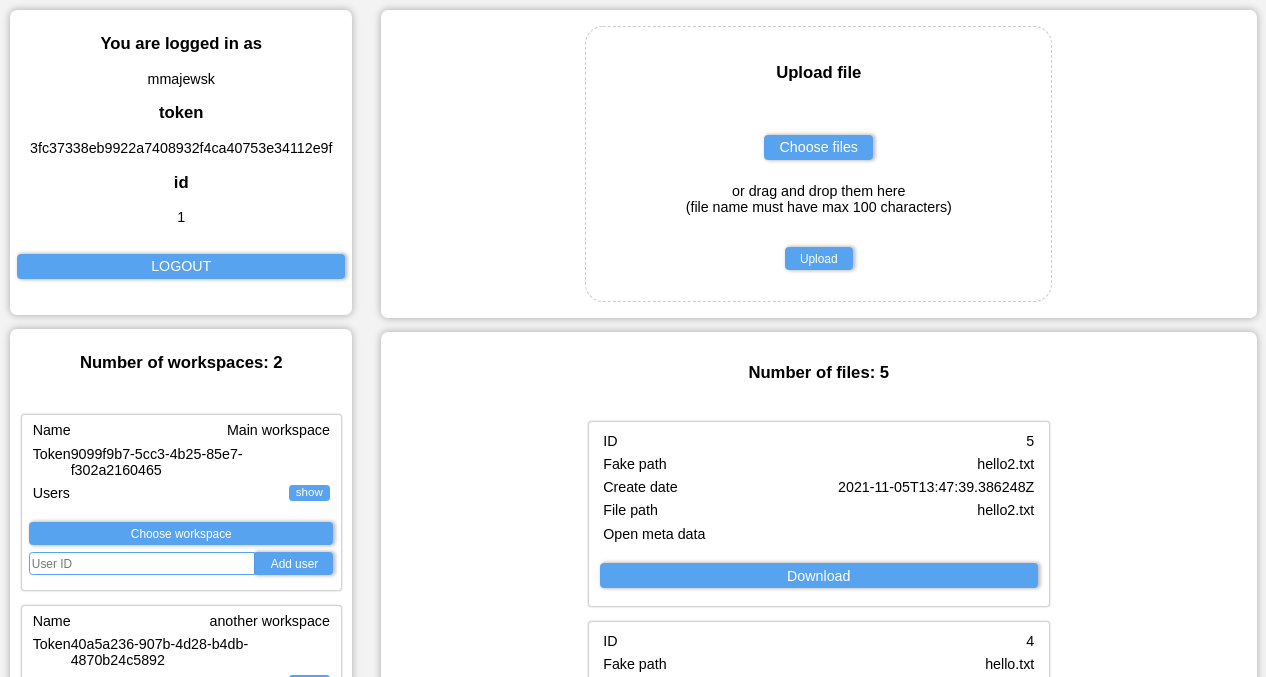
\includegraphics[width=0.9\textwidth]{figures/chapter5/storck/screenshot_web.png}
\caption{Storck's web interface.}
\label{fig:storck-web-interface}
\end{figure}

Storck's web interface is very basic, as it is not meant to be the primary way of interacting with storck.
In Fig. \ref{fig:storck-web-interface}, on the left side, there is a space that contains the user's username, id and user token.
Below that space, there is a list of available workspaces.
Each of the workspaces shows its workspace token and also allows to add users to the workspace.
The two areas on the right side of the screen are devoted to files.
The top area can be used as a drag-and-drop area to upload files to storck.
The lower area lists all of the files contained in the workspace and allows for the download of each using a dedicated button.


\subsection{Storck python client}

Storck python client was created as a separate project and repository to the main Storck project.
To use it, python users can simply install it as a package using a command:

\mintinline{bash}{pip install git+https://gitlab.cern.ch/velo-calibration-software/storck}

or

\mintinline{bash}{pip install storck-client}

\noindent It is a very small and simple package. It is an object-oriented API in python, and users should create and operate on the Storck client object.
The very basic usage is as follows:


\begin{listing}[!ht]
\begin{minted}{python}
from storck client import StorckClient

client = StorckClinet(api_host=..., user_token=..., workspace_token=...)
print(client.get_files())

\end{minted}
\caption{A snippet of code presenting how storck python client can be used.}
\label{listing:storck_client}
\end{listing}

The Storck client constructor accepts three arguments: the HTTP address to the Storck server, user token, and workspace token.
These arguments are optional as, instead the environmental variables can be set, in order to not provide the tokens in plain text.
The client has several methods, which we present in the form of a table (\ref{tab:storck_client}).
For a more detailed description of all of the methods, we refer the reader to the Storck documentation page\cite{storckdock}.


\begin{table}[h!]
\begin{center}
\begin{tabular}{ |c|c| }
\hline
Method & description \\
\hline
auth\_verify & verifies the credentials t\\
set\_workspace\_token & sets the workspace token for the client object\\
create\_workspace & creates new workspace\\
get\_files & outputs list of files in the workspace\\
get\_file & returns all information about given file\\
upload\_file & uploads the contents of the file and its information\\
download\_file & downloads the contents of the file\\
add\_user\_to\_workspace & adds user to workspace\\
\hline
\end{tabular}
\caption{\label{tab:storck_client}Table of available methods of Storck client}
\end{center}
\end{table}

\section{Titania}

Titania is a monitoring framework built with python, Qt \cite{qtframework} and flask\cite{flask}.
Similarly to Storck, Titania is also being adopted at the Velo group for the next LHC runs.
This section will present the design and exemplary uses of the framework.

\subsection{Motivation}
Drawing from the experience of working with monitoring in Run 1 and Run 2, we have proposed a new project for handling the monitoring tasks.
The previous software for the monitoring, although useful, was getting complicated in the development due to the amounts of different uncoordinated changes.
The platform's source code was not well structured, so adding new plots was usually quite the challenge.
This drove us to develop a new platform for monitoring Velo as a python framework.

\subsection{Software Stack}

Python is one of the most popular tools for plotting and visualisation in the scientific community, thanks to packages like Matplotlib\cite{Hunter:2007} or Plotly \cite{plotly}.
Famously, the first image of the black hole \cite{blackhole} was created with python, and visualisation using matplotlib in the first extraterrestrial flight on mars played a significant role \cite{ingenuity}.
Titania was designed with the desktop GUI in mind first (it also contains some web interface capabilities).
So naturally, we used the PyQt library, which interfaces the QtGUI library to python.
QtGUI, in short, provides an easy way to create cross-platform GUI applications.
It is an object-oriented library and implements a system of sockets and connections for action triggering.

\subsection{Framework Design}

As previously stated, one of the key goals of the new system is extensibility and orderliness.
Inspired by Django's concept of implementing MVC in the framework, we define three key components to any monitoring task.

\begin{itemize}
  \item \textbf{Data}
  \item \textbf{Plots}
  \item \textbf{Exploration}
\end{itemize}

Those are fundamental blocks of any monitoring tasks.


\textbf{Data} here is understood in terms of the source of data. Anytime we want to show some data, we need to access them.
There are many ways that this can be done; reading files from a disk, reading a stream of data, receiving data as an HTTP request and others.
This also means a format of the data. Data can be text files of CSV structure, binary files, images or sound recordings.

\textbf{Plots} are the graphical representation of the data. This means linear plots, scatter or histogram and others. Each of the ways of representing the data has its custom options of placement, colours, and other things.

\textbf{Exploration} - one must be able to choose between different data sources and different plot types. If a monitoring service shows only one plot from one data file, it can hardly be a system.


\subsection{Using Titania}

The detailed API can be found online \cite{titaniadoc}; nonetheless, we present here some of the examples of the classes used.
Drawing inspiration from the Django framework, the Titania package contains a script that enables the creation of a Titania project.

\mintinline{bash}{python -m titania start --name ProjectName}

This command will create a folder with the following structure:

\begin{listing}[!ht]
\begin{minted}{text}
ProjectName
|── data/
|── panels/
|── plots/
|── views/
|── main.py
|── config.py
\end{minted}
\end{listing}

This script also contains an exemplary implementation of selected classes.
The whole program can be run using the main.py file.
Each of the subdirectories is devoted to different parts of the framework.


\subsubsection{Data}
\label{sec:titania_data}

All of the data classes created with Titania, are required to subclass \textbf{TitaniaDataInterface}. This requires an implementation of the \textbf{fetch()} method.
The only requirement for the implementation of this method is that it will return any kind of data.
This serves one purpose; all data coming in any shape or form after reading/processing can be sent from this class with a common interface. An exemplary class implementation that gets the temperature data can be found in the listing below (Listing \ref{listing:data}).

\begin{listing}[!ht]
\begin{minted}{python}

import urllib.request
import json
import datetime
from titania.data.data_core import TitaniaDataInterface

class WeatherData(TitaniaDataInterface):
    def __init__(self):
        self.request_string = "https://www.7timer.info/bin/astro.php"+/
        "?lon=6.097&lat=46.241&ac=0&unit=metric&output=json&tzshift=0"

    def fetch(self):
        response = urllib.request.urlopen(self.request_string).read()
        data = json.loads(response)
        temp = [v['temp2m'] for v in data['dataseries']]
        timepoints = [v['timepoint'] for v in data['dataseries']]
        initial_date = datetime.datetime.strptime(data['init'], "%Y%m%d%H")
        exact_timepoints = [initial_date+datetime.timedelta(hours=h) for h
        in timepoints]
        return temp, exact_timepoints
\end{minted}
\caption{Example of Data implementation}
\label{listing:data}
\end{listing}

The implementation above is requesting an open REST API for the weather data, processing it, and returns a list of measurements and a list of time points as python objects.
It can be noticed that this could also be implemented in such a way that the data could be acquired in the constructor of the class and then statically returned from the \textbf{fetch()} method.

\subsubsection{Plots}

The implementation of the Plot in the Titania is slightly more complicated. While the Data component does not depend on the interface used (Web or Desktop GUI), some plots may differ in implementation depending on the interface.

The minimal requirement for a plot is implementation of \textbf{PlotInterface} class.
This requires following methods: \textbf{draw\_plot()}, \textbf{get\_as\_plot\_widget()}.
The first method is used for any drawing action that the plotting library requires.
The \textbf{get\_as\_plot\_widget()} requires returning the \textbf{QtWidget} object.
The output from this function is then used to construct the GUI.
There are already classes implemented in the titania framework that can be used for more specific cases that are described in the documentation of the project.
In general, it is advised to use the \textbf{MplPlot} class for implementing a plot class using matplotlib.


\begin{listing}[!ht]
\begin{minted}{python}
from titania.plots.base_plot import MplPlot

class WeatherPlot(MplPlot):
    def __init__(self, parent=None, view=None, *args, **kwargs):
        MplPlot.__init__(self, parent=parent, view=view)
        self.color = 'blue'

    def draw_plot(self, data=None) -> None:
        self.figure.clear()
        ax = self.figure.add_subplot(self.plot_number)
        temp, timepoints = self.view.data.fetch()
        ax.plot(timepoints, temp, color=self.color)
        self.draw()
\end{minted}
\caption{Example of Plot implementation}
\label{listing:plot}
\end{listing}

This implementation (Listing \ref{listing:plot}) makes a simple matplotlib line plot, using the colour defined in the ``self.color'' attribute.

\subsubsection{Exploration}

This part is strictly connected to the interface. The minimal requirement for implementing the ``Exploration'' in the framework is implementation of the \textbf{ControlPanelInterface} and it's \textbf{get\_control\_panel()} method.
That method must return the ``QWidget'' object containing the widget of the panel.

\begin{listing}[H]
\begin{minted}{python}
from titania.panels import ControlPanelInterface
from PyQt5.QtWidgets import QVBoxLayout, QPushButton

class WeatherControlPanel(ControlPanelInterface):
    def __init__(self, data=None, widget=None):
        self.widget = widget
        self.control_panel = QVBoxLayout()
        self.red = QPushButton("Change to red")
        self.blue = QPushButton("Change to blue")
        self.control_panel.addWidget(self.red)
        self.control_panel.addWidget(self.blue)
        self.red.clicked.connect(self.change_color_to_red)
        self.blue.clicked.connect(self.change_color_to_blue)

    def change_color_to_red(self):
        self.widget.plot.color = 'red'
        self.widget.plot.draw_plot()

    def change_color_to_blue(self):
        self.widget.plot.color = 'blue'
        self.widget.plot.draw_plot()

    def get_control_panel(self):
        return self.control_panel

\end{minted}
\caption{Example of Exploration implementation}
\label{listing:exploration}
\end{listing}

The exemplary implementation (Listing \ref{listing:exploration}) creates a straightforward panel that contains two buttons named ``blue'' and ``red'' (left side of the window in Fig. \ref{fig:titania-weather}).
It is connected using Qt signals to change the ``color'' property of the plot class to the according name of the button and executes the plot drawing action.

\subsubsection{Views}

The View connects Data, Plotting and Exploration. Views should implement \textbf{TitaniaTabInterface}, with \textbf{get\_title()} and \textbf{initiate()} methods.
Since we assume a tabular design of the interface, \textbf{get\_title()} should be returning the name displayed name of the tab.
The \textbf{initate} method is used to start all of the things needed for the view to work.
As it is a very basic requirement, many classes exist that already implement valuable features.
The recommended class to use when making a tab for titania in Qt is \textbf{QtBaseLayoutTab}.
It's implementation requires:
\begin{enumerate}
\item Passing a data class to \textbf{QtBaseLayoutTab} constructor using data argument.
\item Returning a Plot class from \textbf{make\_plot} function
\item Returning title with \textbf{get\_title()} function
\item Returning a Exploration class, which extends \textbf{ControlPanelInterface} \\ with method \textbf{create\_control\_panel()}
\end{enumerate}
The exemplary implementation of the View class is in Listing \ref{listing:view}.


All of those exemplary implementation should be put together in the following directory structure:

\begin{listing}[!ht]
\begin{minted}{text}
ProjectName
|── data/
    - weather_data.py
|── panels/
    ─ weather_panel.py
|── plots/
    ─ weather_plot.py
|── views/
    ─ weather_gui.py
|── main.py
|── config.py
\end{minted}
\end{listing}

All of this makes into a single tab that is depicted in the \ref{fig:titania-weather}.

\begin{listing}[!ht]
\begin{minted}{python}
from panels.weather_panel import WeatherControlPanel
from data.weather_data import WeatherData
from plots.weather_plot import WeatherPlot
from titania.QtGUI.base_tab import QtBaseLayoutTab

class WeatherGUI(QtBaseLayoutTab):
    def __init__(self, parent=None):
        super().__init__(data=WeatherData(), parent=parent)

    def make_plot(self):
        return WeatherPlot(parent=self.parent, view=self)

    def get_title(self):
        return "Weather Plot"

    def create_control_panel(self):
        return WeatherControlPanel(widget=self)

\end{minted}
\caption{Example of View implementation}
\label{listing:view}
\end{listing}

\begin{figure}[h]
\centering
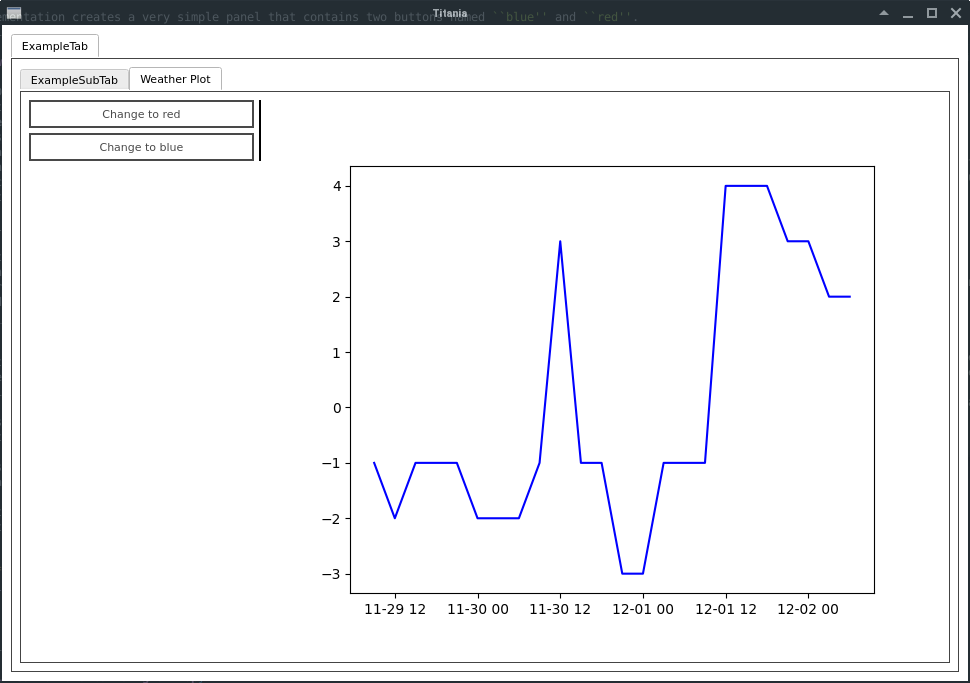
\includegraphics[width=0.7\textwidth]{figures/chapter5/titania/titania_weather_screen.png}
\caption{Exemplary code combined into weather plot view in Titania.}
\label{fig:titania-weather}
\end{figure}

\subsubsection{Optimisation and building on top}

The example in the section above may seem like an excessive amount of code for such a limited functionality.
This may be true for such small projects, but when the number of features grows, such design allows for easy reusability of the already created code.
A case for it may be the following example:
The \textbf{WeatherData} class created in Sec. \ref{sec:titania_data} has a minor flaw: the actual call of \textbf{fetch()} may be pretty slow due to the slow loading time of the HTTP request.
In some cases, the rate of available REST API calls per amount of time is restricted.
Additionally, each time the colour of the plot changes, the \textbf{fetch()} method has to be called one more time, which makes the colour changing feature slow.
One of the methods to deal with this problem could be an implementation that uses the cache to store the API calls and creates new request when a certain timespan is exceeded.
An exemplary implementation of such a class can be seen in the Listing \ref{listing:weather_upgrade}.


\begin{listing}[!ht]
\begin{minted}{python}
class WeatherDataCached(WeatherData):
    def __init__(self):
        WeatherData.__init__(self)
        self.last_check = None
        self.data = None

    def fetch(self):
        now = datetime.datetime.now()
        if self.last_check is None:
            self.last_check = datetime.datetime.now()
        else:
            dif = now-self.last_check
            if  dif.seconds//(5*60) b>= 1:
                self.data=None
                self.last_check = now
        if self.data is None:
            self.data = WeatherData.fetch(self)
        return self.data
\end{minted}
\caption{Example of Exploration implementation}
\label{listing:weather_upgrade}
\end{listing}


The class \textbf{WeatherDataCached} extends the class \textbf{WeatherData}, and adds two attributes \textbf{data} and \textbf{last\_check}.
The  \textbf{data} attribute stores the data coming from the parent \textbf{WeatherData.fetch()} method, and  \textbf{last\_check} contains the last time of the call of that method.
When the time span of 5 minutes is exceeded, the data is refreshed. Otherwise, the data received with the last call of \textbf{WeatherData.fetch()} is returned.

Now, to run a new upgraded version of the program, we need only one additional change seen in Listing \ref{listing:weather_change}.

\begin{listing}[!ht]
\begin{minted}{python}
...
class WeatherGUI(QtBaseLayoutTab):
    def __init__(self, parent=None):
        super().__init__(data=\textbf{WeatherDataCached()}, parent=parent)
...

\end{minted}
\caption{Update to the WeatherGUI class to use cache data}
\label{listing:weather_change}
\end{listing}

As you can see, the final change to the existing code is minimal, and other parts (exploration and plotting) do not need any changes. This proves the robustness of the framework.

\subsubsection{Web app}
Although the feature of enabling a dual interface (both desktop GUI and web) is not yet fully developed, the titania project enables such an option.

In order to do so, the following requirements must be met for a view class:
\begin{itemize}
  \item It must extend both \textbf{TitaniaPlotTab} and the \textbf{WebTab} class
  \item It must contain an member object \textbf{self.plot.figure} of matplotlib's figure type
\end{itemize}

With the usage of example snippets of code from previous sections, the dual interface can be introduced by splitting the \textbf{WeatherGui}, as depicted by Listing \ref{listing:weather_split}.


\begin{listing}[!ht]
\begin{minted}{python}
from panels.weather_panel import WeatherControlPanel
from data.weather_data import  WeatherData, WeatherDataCached
from plots.weather_plot import WeatherPlot
from titania.common.titania_tab import TitaniaPlotTab

class Weather(TitaniaPlotTab):
    def __init__(self, parent=None):
        self.parent = parent
        super().__init__(data=WeatherDataCached())

    def make_plot(self):
        return WeatherPlot(parent=self.parent, view=self)

    def get_title(self):
        return "Weather Plot"from titania.QtGUI.base_tab import QtBaseLayoutTab

class WeatherGUI(Weather, QtBaseLayoutTab):
    def __init__(self, parent=None):
        QtBaseLayoutTab.__init__(self, parent=parent)
        Weather.__init__(self, parent=parent)

    def create_control_panel(self):
        return WeatherControlPanel(widget=self)
\end{minted}


\caption{WeatherGUI class split into two classes}.
\label{listing:weather_split}
\end{listing}
Such split allows for the implementation of the \textbf{WeatherWeb} class (Listing \ref{listing:weather_split}), which will be used for the web interface view.
The implementation in Listing \ref{listing:weather_webclass} implementation inherits the \textbf{Weather} class and \textbf{QtTitaniaWebTab}.
Both provide inheritance valid for the web view.
\begin{listing}[!ht]
\begin{minted}{python}
class WeatherWeb(Weather, QtTitaniaWebTab):
    def __init__(self, parent=None):
        self.parent = parent
        Weather.__init__(self, parent=parent)
        QtTitaniaWebTab.__init__(self)
\end{minted}
\caption{WeatherWeb class}
\label{listing:weather_webclass}
\end{listing}
Additionally, for easier creation of the web view, there is also a possibility of using \textbf{WebMetaclass} (Listing \ref{listing:weather_web_meta}).
\begin{listing}[!ht]
\begin{minted}{python}
from titania.web.base_tab import WebMetaclass

class WeatherWeb(Weather, metaclass=WebMetaclass):
    pass
\end{minted}
\caption{WeatherWeb metaclass}
\label{listing:weather_web_meta}
\end{listing}
Both Listing \ref{listing:weather_web_class} and Listing \ref{listing:weather_web_meta} are good ways of creating the web interface view.
To enable the web interface, a new configuration file must be created ``config\_web.py'' (Listing \ref{listing:weather_web_config}). It should include the new web view class in the dictionary.

\begin{listing}[!ht]
\begin{minted}{python}
from views.weather_gui import WeatherWeb
config = {
    "ExampleTab": [WeatherWeb],
  }
\end{minted}
\caption{Config file for the web interface.}
\label{listing:weather_web_config}
\end{listing}

Next, the config dictionary should be imported and executed in a new ``main\_web.py'' (Listing \ref{listing:weather_web_main}) file that will start a small web server and host the interface on the \href{http://localhost:5000}{http://localhost:5000}.

\begin{listing}[!ht]
\begin{minted}{python}
import config_web
from titania.web.main_window import MainWindow

if __name__ == '__main__':
    main_window = MainWindow(tab_config=config_web.config)
    main_window.run()}
\end{minted}
\caption{The main file for the web interface example.}
\label{listing:weather_web_main}
\end{listing}


\begin{figure}[H]
\centering
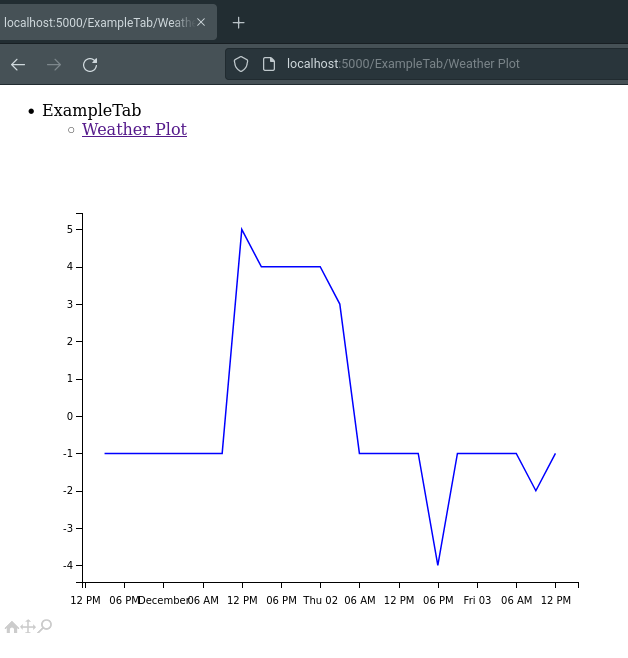
\includegraphics[width=0.7\textwidth]{figures/chapter5/titania/titania_weather_web.png}
\caption{A screenshot of the exemplary titania web interface app }
\label{fig:titaniawebinterface}
\end{figure}

All of the code presented in this section allows for simultaneously running the Web and Desktop interfaces.
This significantly reduces the amount of code needed to run both the desktop version and the web interface.

\section{Conclusions}

Titania is a versatile monitoring framework, and Storck should create a reliable backbone for the calibration data in the next runs of Velo at LHCb.
As of the time of writing, it is being introduced, beside Velo, to another of the silicon systems at LHCb UT - Upstream Tracker.
Both projects are open source and fully available online.
They solve not only the specific problems of the LHCb but also provide more general solution to the problems that might occur in other areas or physics experiments.
Titania was presented in its earlier stages at the PyHep conference in 2020.
Hopefully, the upcoming year will prove in-vivo the value of both of the projects and promote its uses in other experiments.

%%% Local Variables:
%%% mode: latex
%%% TeX-master: "../dissertation"
%%% TeX-engine: xetex
%%% End:
